% Requires packages: booktabs, tikz
% Auto-generated polarization index report: run\_Phase3\_r1\_2026-05-25\_23-19-21
\begin{table}[ht]
\centering
\small
\begin{tabular}{llrrrr}
\toprule
Agent A & Agent B & WR(A,B) (\%) & |WR-50| & DeckStd & Polarization \\
\midrule
21 glebokosciowy & MyAgentSebastianMiller2Naive & 47.36 & 2.64 & 11.68 & 14.32\\
\bottomrule
\end{tabular}
\caption{Polarization index for run\_Phase3\_r1\_2026-05-25\_23-19-21: $\mathrm{PI}(A,B)=|WR(A,B)-50|+\sigma_{deck}(A,B)$. Higher = stronger and/or more deck-dependent matchup.}
\end{table}

\begin{figure}[ht]
\centering
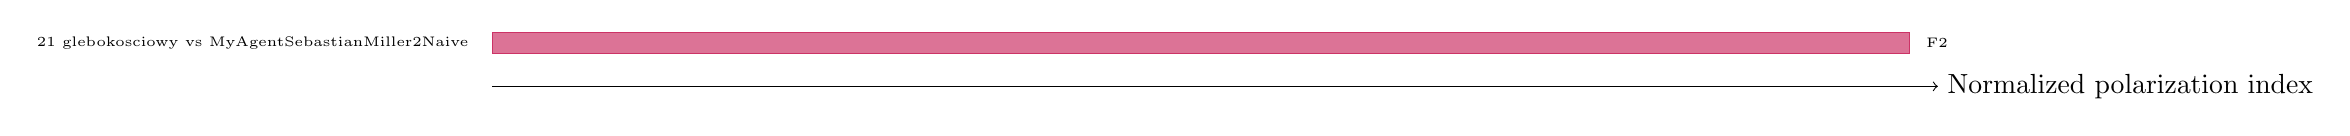
\begin{tikzpicture}[x=0.18cm,y=0.55cm]
\draw[->] (0,0) -- (102,0) node[right] {Normalized polarization index};
\filldraw[fill=purple!55, draw=purple!80] (0,1-0.25) rectangle (100.00,1+0.25);
\node[anchor=east, font=\tiny] at (-1,1) {21 glebokosciowy vs MyAgentSebastianMiller2Naive};
\node[anchor=west, font=\tiny] at (100.00+0.5,1) {F2};
\end{tikzpicture}
\caption{Polarization ranking for run\_Phase3\_r1\_2026-05-25\_23-19-21 (bars normalized to the maximum PI in this run).}
\end{figure}
